\subsection{pT smearing}

当我们通过模拟的方法得到一对$e^+$和$e^-$的动力学信息之后,在将其重建成电子对之前我们需要对其横动量的分布添加pT smearing来反应探测器的分辨对最后质量分布的影响。在STAR官方的模拟(embedding)当中,已经添加了一定的探测器对径迹动量的影响,但是embedding当中的模拟结果和实际情况相比过于精确地反映了探测器的分辨率,需要我们对其参数来进行调整来更好地反应探测器的影响。

在embedding的样本当中,可以得到$\sigma_{p_T}/p_T = \frac{p_T^{RC}~-~p_T^{MC}}{p_T^{RC}}$在不同$p_T$区间内的分布。在拟合这个分布可以得到$p_T$的分辨率$\sigma_{p_T}/p_T$随$p_T$变化的曲线,如图\ref{fig:pT_res_embd}所示。其中拟合曲线为式\ref{eq:pT_res}。当得到a的值之后,接下来要做的是对a进行扫描从而得到最佳的a的值。
\begin{equation}
    \label{eq:pT_res}
    \delta_{p_T} = \sqrt{a^2 p_T^2 + b^2}
\end{equation}

\begin{figure}[htb]
    \begin{center}
    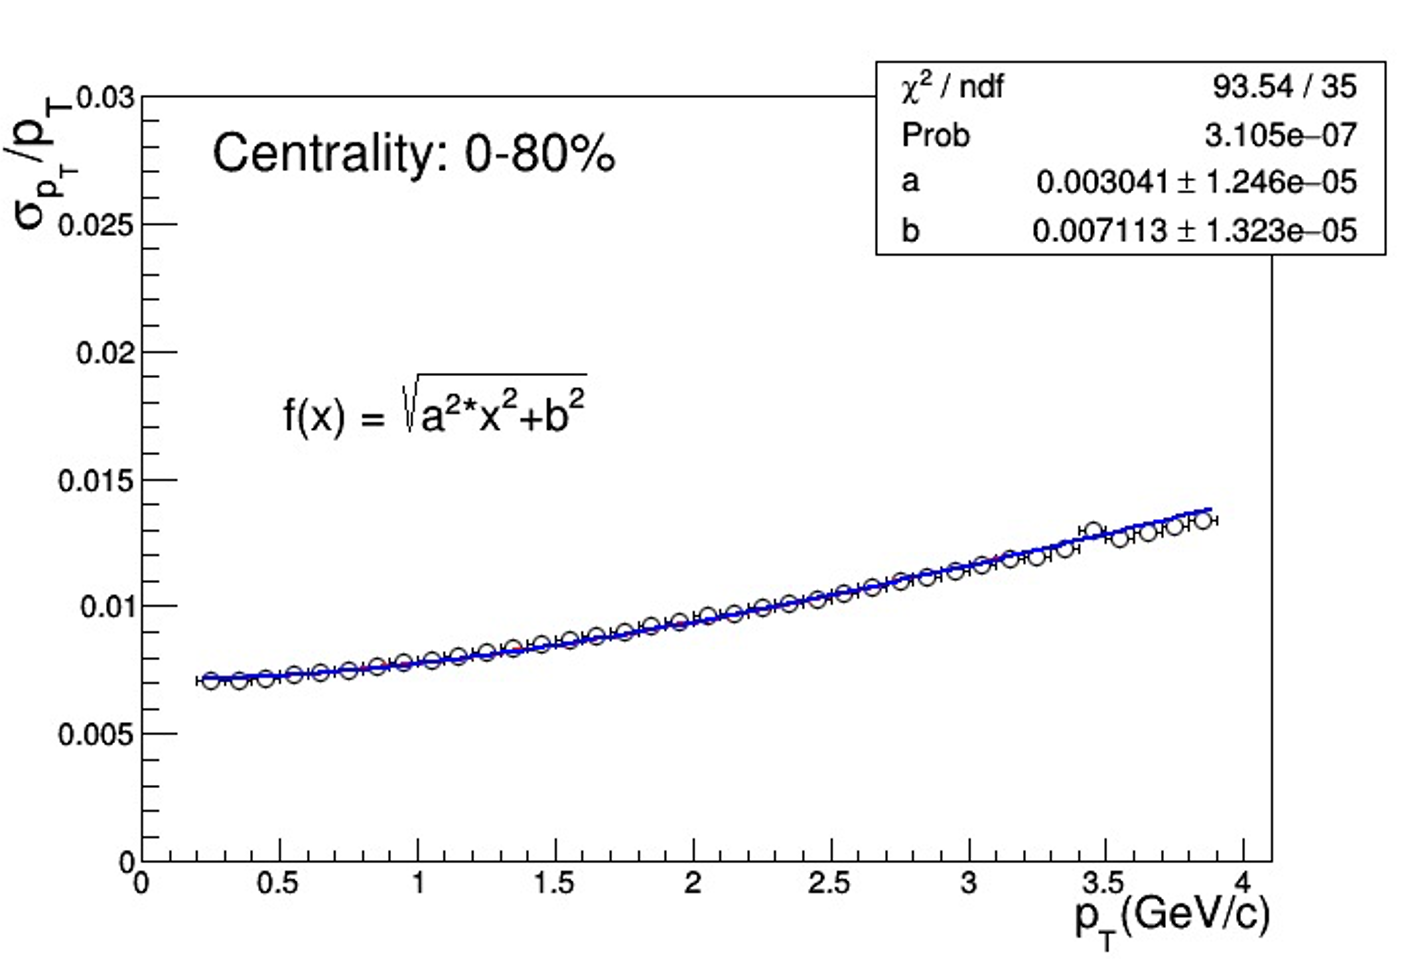
\includegraphics[width=0.8\textwidth,clip]{figures/Chapter4/pT_res_embd.png}
    \end{center}
    \caption[横动量分辨率随横动量变化示意图]{0-80\%中心度下横动量分辨率随横动量变化示意图,并通过拟合得到$\sigma_{p_T}/p_T$随$p_T$变化的曲线,拟合结果在图中标出。}
    \label{fig:pT_res_embd}
\end{figure}

为了对分辨率进行扫描,我们选取${\rm J/\psi}$的峰作为标定的参考。通过调整a的值产生在不同的a的情况下的${\rm J/\psi}$模拟的分布,再用这个模拟的分布去拟合数据中重建出来的${\rm J/\psi}$的分布。使拟合结果的$\chi^2$最小的a的值就是我们最后在模拟当中使用的a的值。扫描结果如图\ref{fig:Chi2_TuneA}所示。在不同中心度下的a的值见表\ref{tab:a}。
\begin{figure}[htb]
    \begin{center}
    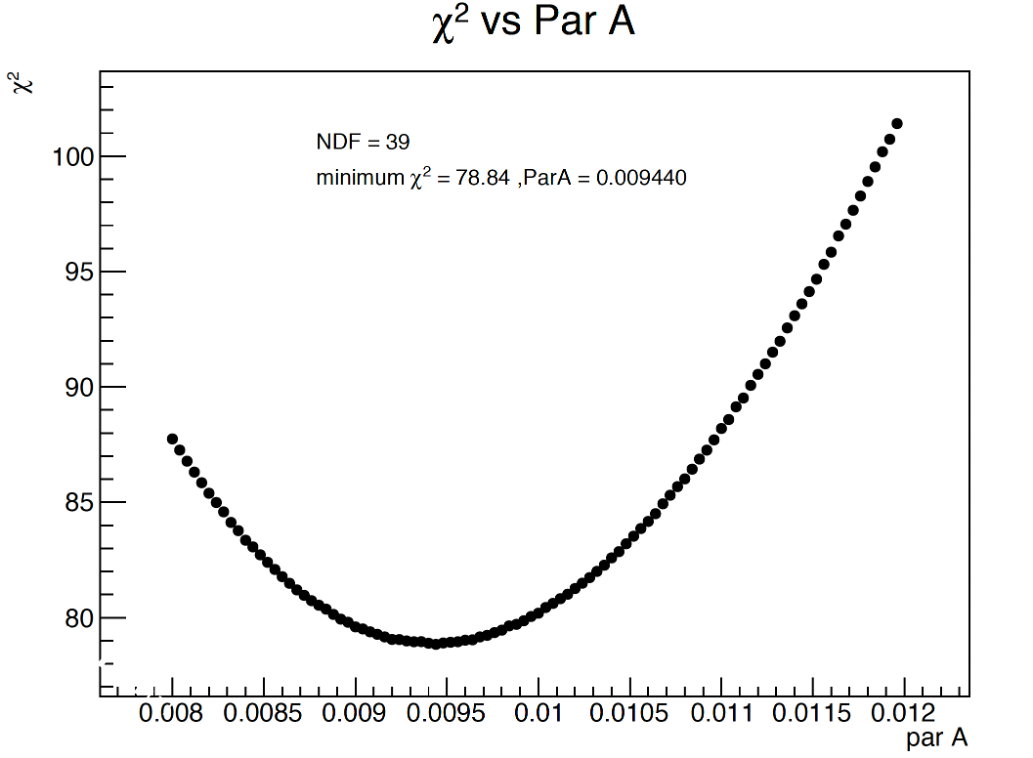
\includegraphics[width=0.8\textwidth,clip]{figures/Chapter4/Chi2_TuneA.png}
    \end{center}
    \caption[不同参数a时模拟样本拟合数据的$\chi^2$分布]{寻找最佳参数a时不同a下$\chi^2$的值}
    \label{fig:Chi2_TuneA}
\end{figure}
\begin{table}[h!]
    \centering
    \caption{\sNN = 54.4 GeV 金-金对撞中不同中心度下a的值}
    \label{tab:a}
    \begin{tabularx}{0.8\textwidth} {
    | >{\centering\arraybackslash}X  |>{\centering\arraybackslash}X | }
    \hline
    Centrality & a \\
    \hline
    0-80\% & 0.006450 \\
    \hline
    0-10\% & 0.005600 \\
    \hline
    10-40\% & 0.007700 \\
    \hline
    40-80\% & 0.008250 \\
    \hline
    \end{tabularx}
\end{table}